\documentclass[12pt]{exam}



\usepackage{graphicx}% Include figure files
\usepackage{dcolumn}% Align table columns on decimal point
\usepackage{bm}% bold math
\usepackage{latexsym}
\usepackage{amsmath,amssymb,amsthm,amsfonts}
\usepackage{subfigure}

\begin{document}
\pagestyle{head} \extraheadheight{1in}\runningheadrule
\firstpageheader{$\mbox{}$\\DATE: March 3, 2009\\PAPER NO.: - \\
DEPARTMENT $\&$ COURSE NO.: MATH 3820\\EXAMINATION: Intro. Math. Modelling}{\bf UNIVERSITY OF MANITOBA\\
$\mbox{}$
\\$\mbox{}$ \\ $\mbox{}$\\$\mbox{}$}{$\mbox{}$\\Test 1\\ PAGE NO.: \thepage\ of \numpages\\TIME: 120
minutes\\ EXAMINER: J. Arino}\runningheadrule
\runningheader{$\mbox{}$\\DATE: March 3, 2009\\PAPER NO.: - \\
DEPARTMENT $\&$ COURSE NO.: MATH 3820\\EXAMINATION: Intro. Math. Modelling}{\bf UNIVERSITY OF MANITOBA\\
$\mbox{}$
\\$\mbox{}$ \\ $\mbox{}$\\$\mbox{}$}{$\mbox{}$\\Test 1\\ PAGE NO.: \thepage\ of \numpages\\TIME: 120
minutes\\ EXAMINER: J. Arino} \vspace{-2.5cm}
\begin{center}
\begin{tabular}{cp{15.5cm}}
\hline
&\\
\end{tabular}
\end{center}
%\footer{}{Page \thepage\ of \numpages}%
%{\iflastpage{End of exam.}{Please go on to the next page\ldots}}

\addpoints

This is a 120 minutes exam, with \numquestions\; questions for a total of \numpoints\; marks. Lecture Notes are allowed.
{\sc Please show your work clearly.} A correct answer without explanation will not get full marks.
\vspace{0.1cm}

\begin{center}
\begin{tabular}{cp{15.5cm}}
\hline
&\\
\end{tabular}
\end{center}

\printanswers



\begin{questions}

\question[10]
The dynamics of a population of birds (measured in thousand) is described by the equation
\[
\frac{dP}{dt}=4P(1-8P^3).
\]
\begin{parts}
\part Find the equilibria.
\begin{solution}
This is a continuous time system. 
We write
\[
P'=f(P):=4P(1-8P^3).
\]
Equilibria satisfy $f(x)=0$. Clearly, $4P=0$, i.e., $P=0$, or $1-8P^3=0$, that is, $P=1/2$.
\end{solution}
\part Determine the local stability of each equilibrium.
\begin{solution}
The local stability depends on the sign of $f'$ at the equilibria. We have $f'(P)=4(1-8P^3)+4P(-8\times 3P^2)=4-128P^3$. Thus $f'(0)=4>0$, so $0$ is unstable, and $f'(1/2)=-12<0$, so $1/2$ is locally asymptotically stable.
\end{solution}
\end{parts}



\vskip0.5cm
\question[10]
The population (measured in billions) of insects in generation $t$ is described as follows
$$P_{t+1}=P_t e^{4(1-3P_t)}$$
\begin{parts}
\part Find all fixed points.
\begin{solution}
We define
\[
P_{t+1}=f(P_t):=P_t e^{4(1-3P_t)}.
\]
This is a discrete-time system, so equilibria satisfy $f(p)=p$. Thus we solve
\[
p=pe^{4(1-3p)}.
\]
We find $p=0$ and $1=e^{4(1-3p)}$. The latter gives $\ln 1=4(1-3p)$, that is, $1-3p=0$. Thus there are two equilibria, $p=0$ and $p=1/3$.
\end{solution}
\part Determine the local stability of each fixed point.
\begin{solution}
This is a discrete-time system, so the local stability of the equilibria is determined by whether $|f'(p)|<1$ or not.

We have
\[
f'(p)=(1-12p)e^{4(1-3p)}.
\]
So, at $p=0$, we have $|f'(0)|=e^4>1$, 0 is an unstable equilibrium. At $p=1/3$, $|f'(1/3)|=|-3e^0|=3>1$, so $1/3$ is also unstable.
\end{solution}
\end{parts}




\vskip0.5cm
\question[20]
Assume that an insect population, $x(t)$, is controlled by a natural predator population, $y(t)$. We make the following assumptions:
\begin{itemize}
\item In the absence of predators, the dynamics of the insects is governed by a logistic equation.
\item Preys and predators meet at a rate that is of mass action type.
\item When a contact takes place, the probability per contact that a prey dies is $k_1$. [Hint: think of mass action contact in an epidemic model.]
\item These contacts lead to an increase of the predator population with rate $k_2$.
\item The predators are subject to natural death at the per capita rate $d$.
\end{itemize}
\begin{parts}
\part Write a model describing the interaction of the 2 populations.
\begin{solution}
The most obvious model:
\begin{subequations}\label{sys:3}
\begin{align}
x' &= rx\left(1-\frac xK\right)-k_1xy \label{sys:3x} \\
y' &= k_2xy-dy. \label{sys:3y}
\end{align}
\end{subequations}
This is considered with initial conditions $x(0),y(0)\geq 0$.
\end{solution}
\part Study the model you have written: is it well-posed, what are its equilibria (and when are they realistic), can you determine the stability of these equilibria?
\begin{solution}
First of all, the right hand side in \eqref{sys:3} is a $C^1$ function (it is actually $C^\infty$, as it consists of two multivariate polynomials). This implies that solutions exist and are unique.

Suppose $x(t)=0$ for some $t$. Then $x'=0$ for all subsequent $t$. By uniqueness of solutions, this means that $x(t)=0$ for all $t\geq 0$, that is, $x(0)=0$.
Similarly, $y(t)=0$ for some $t$ implies that $y(0)=0$.
As a consequence, the solutions can never become negative if they start nonnegative.

Equilibria are found by solving 
\begin{subequations}\label{sys:3_EP}
\begin{align}
0 &= rx\left(1-\frac xK\right)-k_1xy \label{sys:3x_EP} \\
0 &= k_2xy-dy. \label{sys:3y_EP}
\end{align}
\end{subequations}
From \eqref{sys:3y_EP}, $y=0$ or $k_2x=d$, that is, $x=d/k_2$. Subsituting $y=0$ into \eqref{sys:3x_EP} gives the classical logistic equation, which we know to have $x=0$ and $x=K$ for equilibria. So we have two equilibria, $(x,y)=(0,0)$ and $(x,y)=(K,0)$, which we call, respectively, $E_1$ and $E_2$. Now, substituting $x=d/k_2$ into \eqref{sys:3x_EP} gives
\[
r\frac{d}{k_2}\left(1-\frac{\frac{d}{k_2}}K\right)-k_1\frac{d}{k_2}y=0,
\]
that is,
\[
\frac{rd}{k_2}\left(1-\frac{d}{k_2K}\right)=\frac{dk_1}{k_2}y,
\]
which gives
\[
y=\frac{k_2}{dk_1}\frac{rd}{k_2}\left(1-\frac{d}{k_2K}\right)
=\frac{r}{k_1}\left(1-\frac{d}{k_2K}\right).
\]
So the last equilibrium is $E_3$, given by
\[
(x,y)=\left(\frac{d}{k_2},\frac{r}{k_1}\left(1-\frac{d}{k_2K}\right)\right).
\]
This equilibrium is (biologically) relevant only if $1-d/(k_2K)>0$, or, in other words, if $k_2K-d>0$.

To determine the stability of the equilibria, we need to determine if all (the two, here) eigenvalues of the Jacobian have negative real parts (local asymptotic stability) or if there is an eigenvalue with a positive real part.
The Jacobian, evaluated at an arbitrary point $(x,y)$, takes the form
\[
J=\begin{pmatrix}
r-k_1y-2\dfrac rK x & -k_1x \\
k_2 y & k_2x-d
\end{pmatrix}.
\]
At $(x,y)=(0,0)$, we have 
\[
J=\begin{pmatrix}
r & 0 \\
0 & -d
\end{pmatrix},
\]
thus eigenvalues are $-d$ and $r>0$ and the equilibrium $(0,0)$ is unstable.
At $(x,y)=(K,0)$,
\[
J=\begin{pmatrix}
-r & -k_1K \\
0 & k_2K-d
\end{pmatrix},
\]
and eigenvalues are $-r$ and $k_2K-d$. So the equilibrium $(K,0)$ is locally asymptotically stable if $k_2K-d<0$, and unstable otherwise. [Remark that this means that if $E_3$ exists, $E_2$ is unstable, and if $E_2$ is locally asymptotically stable, $E_3$ does not exist.] Finally, at the last equilibrium,
\[
J_{E_3}=\begin{pmatrix}
-\dfrac{rd}{k_2K} & -\dfrac{k_1d}{k_2} \\
\dfrac{r}{k_1K}(k_2K-d) & 0
\end{pmatrix}.
\]
Eigenvalues of $J_{E_3}$ satisfy
\[
|J_{E_3}-\lambda\mathbb{I}|=\left|\begin{matrix}
-\dfrac{rd}{k_2K}-\lambda & -\dfrac{k_1d}{k_2} \\
\dfrac{r}{k_1K}(k_2K-d) & -\lambda
\end{matrix}
\right|=0.
\]
This gives the characteristic polynomial
\[
P(z)=z^2+\frac{rd}{k_2K}z+\frac{rd}{k_2K}(k_2K-d).
\]
The roots of $P(z)$ are the eigenvalues of $J_{E_3}$. We compute the discriminant
\[
\Delta:=\frac{rd}{k_2K}-4\frac{rd}{k_2K}(k_2K-d)=\frac{rd}{k_2K}(1-4(k_2K-d)).
\]
Roots of $P$ take the form
\[
\frac{-\frac{rd}{k_2K}\pm\sqrt{\Delta}}2.
\]
If $\Delta<0$, then the roots are complex with real part given by the part outside of the square root (thus the real parts are negative). In that case, the equilibrium is locally asymptotically stable.

Now consider the case where $\Delta\geq 0$. The root taking the form
\[
\frac{-\frac{rd}{k_2K}-\sqrt{\Delta}}2
\]
is negative. On the other hand, the root taking the form
\[
\frac{-\frac{rd}{k_2K}+\sqrt{\Delta}}2
\]
is positive if
\[
-\frac{rd}{k_2K}+\sqrt{\Delta}>0.
\]
This is equivalent to
\[
\frac{rd}{k_2K}<\sqrt{\Delta},
\]
that is,
\[
\left(\frac{rd}{k_2K}\right)^2<\Delta.
\]
In other words, if
\[
\left(\frac{rd}{k_2K}\right)^2<\frac{rd}{k_2K}(1-4(k_2K-d)),
\]
that is, if
\[
\frac{rd}{k_2K}<1-4(k_2K-d),
\]
then $E_3$ is unstable. Otherwise, $E_3$ is locally asymptotically stable.
\end{solution}
\part Assume that an insecticide is used to reduce the population of insects, but it is also toxic to the predators; hence, the poison kills both preys and predators at rates proportional to their respective populations. Modify your model from (a). [For bonus marks, you may want to see how this modifies the analysis you carried out in (b).]
\begin{solution}
The most obvious model:
\begin{subequations}\label{sys:4}
\begin{align}
x' &= rx\left(1-\frac xK\right)-k_1xy-\delta_1x \label{sys:4x} \\
y' &= k_2xy-dy-\delta_2 y. \label{sys:4y}
\end{align}
\end{subequations}
This is considered with initial conditions $x(0),y(0)\geq 0$.
\end{solution}

\end{parts}



\vskip0.5cm
\question[10]
Consider the difference equation 
\[
x_{t+1}=f(x_t)
\]
with graph shown in the figure below
\begin{center}
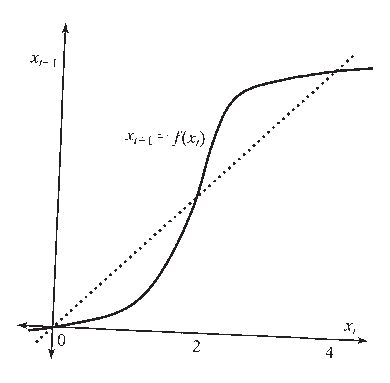
\includegraphics[width=.7\textwidth,,angle=3]{FigureTest1}
\end{center}
\begin{parts}
\part Find all fixed points. 
\begin{solution}
Fixed points are found at the intersections of $f$ with the line $y=x$. So the equilibria are 0, 2 and 4.
\end{solution}
\part Determine the local stability of each fixed point. [Hint: what does the stability condition imply, in terms of the slope of $f$?]
\begin{solution}
Saying that $|f'(p)|<1$ is equivalent to saying that the slope of $f$ at the point $p$ is less than 1 (in absolute value). So if the slope is between that of the line $y=x$ (at the top) and the line $y=-x$ (at the bottom), the equilibrium is locally stable, whereas if the slope is above or below these lines, the equilibrium is unstable. 

So the equilibria 0 and 4 are locally stable, and the equilibrium 2 is unstable.
\end{solution}
\end{parts}


%\question[6]
%Show that the $2-$cycle
%$$\bar x_{1,2}=\frac{1\pm \sqrt{4r-3}}{2}$$
%of the difference equation $x_{t+1}=r-x_t^2$ is unstable if $r> 5/4$.
%\newpage



%Consider the differential equation: $\frac{dy}{dx}=y^2-4$ (Do not
%solve the equation)
%\begin{enumerate}
%\item Is the above differential equation linear or nonlinear,
%autonomous or non-autonomous? Explain.
%\item Find the equilibrium solutions.
%\item Among the 3 direction fields shown on the next page, select
%the one corresponding to the above differential equation.
%\item Use the appropriate direction field to draw an approximate
%integral curve that satisfies $y(0)=0$.
%\item  What is the behavior of your solution in part 4 as $x$ goes
%to $+\infty$; in other words what is $\lim \limits_{x\rightarrow
%\infty}y(x)$?
%\end{enumerate}
%\begin{figure}[ht]
%\centering \subfigure[]{
%\includegraphics[width=.49\textwidth]{Figure1}}
%\subfigure[]{
%\includegraphics[width=.49\textwidth]{Figure2}}
%\subfigure[]{
%\includegraphics[width=.49\textwidth]{Figure3}}
%\end{figure}



%\section*{Question 2} \marginpar{[11]}
%Consider the differential equation: $x\frac{dy}{dx}+y=x^2$
%\begin{enumerate}
%\item Find the general solution of the above differential equation.
%\item What is the interval of validity of solutions?
%\end{enumerate}


%\section*{Exercise 3}
%Consider the differential equation: $\frac{dy}{dt}=ty+t$
%\begin{enumerate}
%\item Show that $y=-1$ is a solution of the above differential equation.
%\item Find the general solution of the above differential equation.
%\end{enumerate}

%\section*{Question 3}\marginpar{[14]}
%Consider the differential equation:
%$\frac{dy}{dx}=-\frac{1}{2}xy^3(1+x^2)^{-1/2}$
%\begin{enumerate}
%\item Show that $y(x)=0$ is a solution of the above differential equation.
%\item Find the general solution of the above differential equation.
%\item Find the solution that satisfies $y(0)=1$.
%\end{enumerate}

%\newpage
%\section*{Question 4}\marginpar{[11]}
%A population of butterflies in a forest increases at a rate $r$
%proportional to the total population. Initially, there are $20,000$
%butterflies, and birds eat $1,000$ butterflies per days.
%\begin{enumerate}
%\item Construct a mathematical model (\emph{i.e.}, differential equation and initial condition) to determine the population of
%butterflies in the forest at any time. Explain your variables,
%parameters and the units used. (Do not solve the equation)
%\item In the
%absence of predators (\emph{i.e.}, with no birds), biologists
%observe that the population triples each week. Calculate the rate of
%birth $r$ of butterflies in the forest (leave your answer with
%logarithms).
%\end{enumerate}




\end{questions}
\end{document}
